\section{Appendix}


\section{Solution Algorithm}

\subsection*{Computing the stationary equilibrium for the Pre-epidemic Stage 0}

\noindent \textbf{\textit{Algorithm No.1}: Computation of the stationary equilibrium:}\\

\noindent\textit{Step 1: Make initial guesses of price $p$ and interest rate $r$.\\
Step 2: Compute the agents decision rules.\\
Step 3: Compute the stationary distribution of assets (follow Algorithm No.2).\\
Step 4: Compute aggregate assets demand and aggregate sex demand. Check the aggregate consistency conditions.\\
Step 5: If conditions are not met, update $p$ and $r$ and return to Step 2.
}\\

Keep in mind that \textit{Algorithm No.1} is generic enough so that it can also be applied to compute the stationary equilibrium of any stage of the HIV epidemic.\\

For the computation of the decision rules I make use of value function iteration with linear interpolation as described in any computational methods text book\footnote{Refer to \cite{mauss}, \cite{judd}, \cite{sargent}}. For the value function iteration procedure it is necessary to choose a grid over the asset space $A=\{a_{1}=a_{min},...,a_{n}=a_{max}\}$ where $a_{min}$ and $a_{max}$ are the values chosen in the calibration. \\

\noindent\textbf{\textit{Algorithm No.2}: Computation of the invariant distribution:}\\

\noindent\textit{Step 1: Choose a grid over the asset space $A=\{a_{1}=a_{min},...,a_{n}=a_{max}\}$.\\
Step 2: Set a time iteration counter $t=0$ and choose an initial (discrete) density function $\phi_{0}(a,e,g,s)$ over the state space.\\
Step 3: Initialize $\phi_{t+1}(a',e,g,s')$\footnote{$\phi_{t+1}$ is of dimensions $n\times (m*w*q)$, where $m=2$, $w=2$ and $q=2$ since education, type and stochastic states can only be of two sorts.} and compute the optimal next period wealth $a'$ with the help of the decision rule.\\
Step 4: For all $a'\in A$, $e \in E$, $g \in G$ and $s \in S$compute the following expression:}
\begin{align}\label{eq:10}
    \phi_{t+1}(a',e,g,s')=\sum_{a,e,s}\sum_{s'|s}\textbf{1}_{a'\in\mathcal{A}}\gamma_{e}\pi(s'|s)\phi_{t}(a,e,g,s) + \psi_{e}\phi_{t}(a',e,g,s')
\end{align}
\textit{
Step 5: If $|\phi_{t+1}-\phi_{t}|<exp(-12)$ stop, otherwise set $\phi_{t}=\phi_{t+1}$ and return to Step 3.}\\

For simplicity reasons the grid chosen for \textit{Algorithm No.2} is the same as the grid chosen for the value function iteration procedure in \textit{Algorithm No.1}, otherwise if the grid would be finer it would be necessary to include the probabilities of $a'(a,e,g,s)$ falling between the respective points in the grid.\\

For \textit{Step2} of \textit{Algorithm No.2} I choose the uniform distribution as the initial values of the distribution. The algorithm should converge regardless of the choice of the initial distribution.


\subsection*{Computing the stationary equilibrium for Stage 1}

\textbf{Solving the Miopic stage}\\
Computation of transition dynamics to a new steady state at every point in time.\\
\noindent \textbf{\textit{Algorithm No.3}: Computation of the Myopic stage:}\\


We are after a sequence of $g_1$. To get each of them we need to solve for the entire transition.

At each period $\tau \in \{T_0+1,..., \infty\}$, agents get a permanent unexpected shock to $\gamma_m$ and $\pi_m$. Then, we need to solve the following algorithm %for each period $t$, that is, every time (which is every period) individuals receive an unexpected shock:\\

\begin{itemize}
\item Step 0: Set $\tau=T_0+1$,
\item Step 1: Compute the recursive stationary equilibrium of the Myopic stage associated with the new $\gamma_m$ and $\pi_m$.
\item Step 2: Choose a very large number of transition  periods $(T-\tau)$.
\item Step 3: Compute the equilibrium transition dynamics from the stationary equilibrium in item 1 (i.e., at $T$) to the  equilibrium in period $\tau$. We compute this standardaly going backwards.
\item Step 4: Stop if $\tau=T_1$
\item Step 5: Replace $\tau=\tau+1$ and go back to Step 1.
\end{itemize}


\subsection*{Computing the stationary equilibrium for Stage 2}
\noindent \textbf{Solving the Maturity of the Epidemic}

Computation of the transition dynamics by guessing a finite-time path for prices.\\

\noindent \textbf{\textit{Algorithm No.3}: Computation of the transition to the Maturity Stage:}\\

\begin{itemize}
\item Step 1: Choose the number of transition periods ($T_2-T_1$) that go from the last  period in Stage 1 (HIV Myopia) ($t=T_1$) to the recursive stationary equilibrium of Stage 2 of the epidemic (HIV Maturity) ($t=T_2$).
\item Step 2: Compute the recursive stationary equilibrium of Stage 2 of the epidemic. This stationary equilibrium is associated with $\lim_{t \rightarrow \infty }\widetilde{\rho}_{e,t}=\rho$. That is, in the stationary equilibrium both education groups have completed learning of the true probability of how HIV risk as a function of sex.
\item Step 3: Guess a time path for the prices $p_{t}$ and $r_{t}$, and a time path for beliefs $\widetilde{\rho}_{e,t}$ by education group.
%The values of these variables in the first period $t = 0$ and last period $t = T$ are implied by the last distribution of the myopic stage of the epidemic and the recursive stationary equilibrium associated with $\widetilde{\rho}_{e,t}=\rho$, i.e., complete learning of the true probability of HIV infection for both education groups.
%\item Step 4: Make an initial guess of $\widetilde{\rho_{e,t}}$ for each education group. and iterate on Bayes rule to generate an exogenous learning path for $ \rho_{t}$ until $T$.
\item Step 5: Compute the equilibrium policy (and value) functions iterating backwards in time, $t = T_2-1,...,T_1$.
\item Step 6: Simulate the evolution of the distribution with the help of the optimal policy functions and the initial distribution for the transition from $t = T_1$ to $t = T_2$.
\item Step 7: Compute the time path of net asset level and excess demand for sex. If markets don't clear along the path, then return to step 3.
\item Step 8: Compare the simulated distribution  with the stationary distribution function. If they are not the same try increasing the horizon $T$.
\end{itemize}


%\subsection*{Computing the dynamics for the pre-epidemic stage}













\subsection{Pre-Epidemic graphs}
\begin{figure}[H]
\caption{Policy Functions Educated Buyers}
\hspace{-2.0cm}
\begin{center}
\begin{tabular}{cc}
\multicolumn{1}{c}{(a) Value function} &  
\multicolumn{1}{c}{(b) Assets function} \\
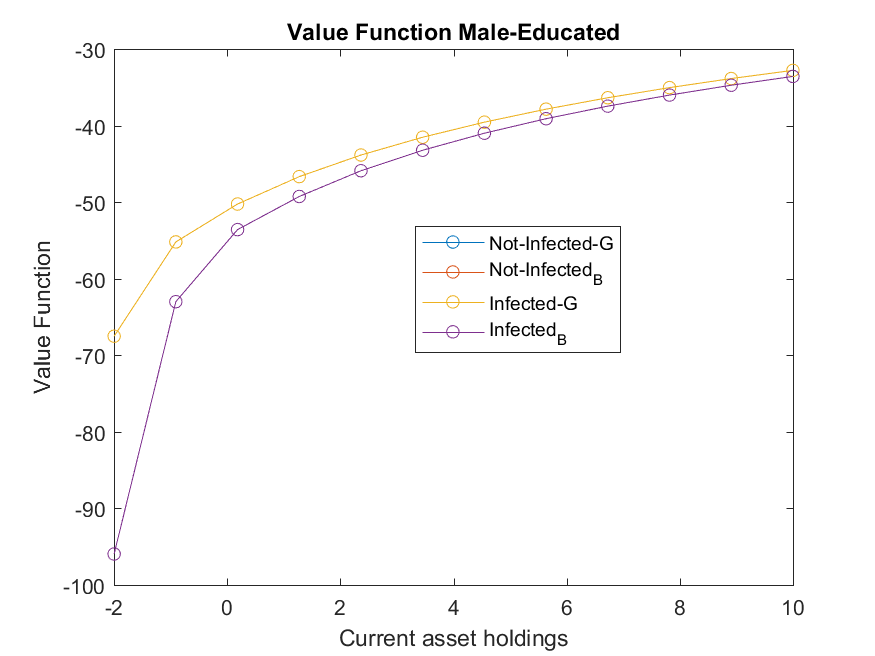
\includegraphics[angle=0,width=.5\textwidth]{figures/FIG1.png}   & 
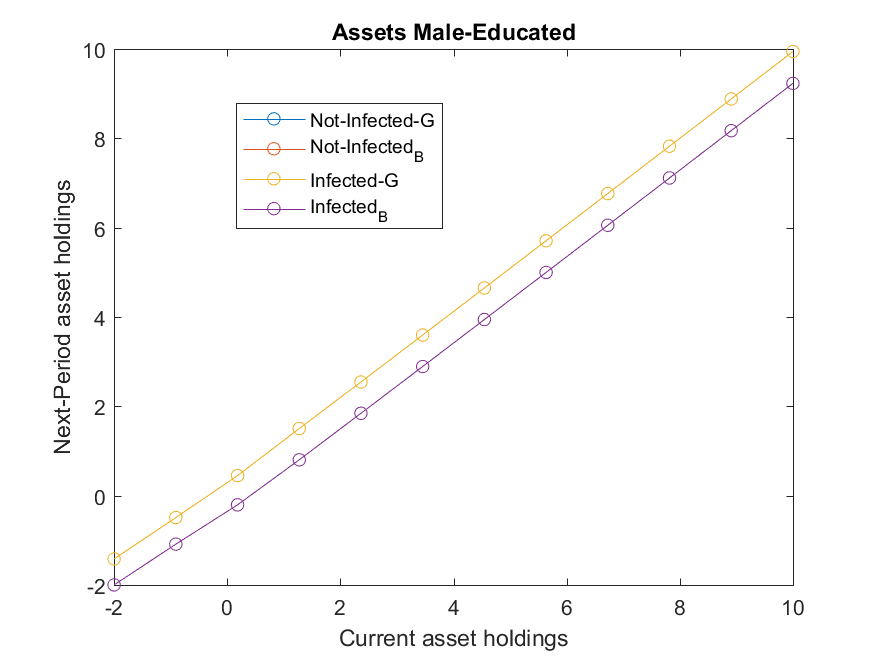
\includegraphics[angle=0,width=.5\textwidth]{figures/FIG3.png} \\
\multicolumn{1}{c}{(c) Consumption function} &  
\multicolumn{1}{c}{(d) Sex consumption function } \\
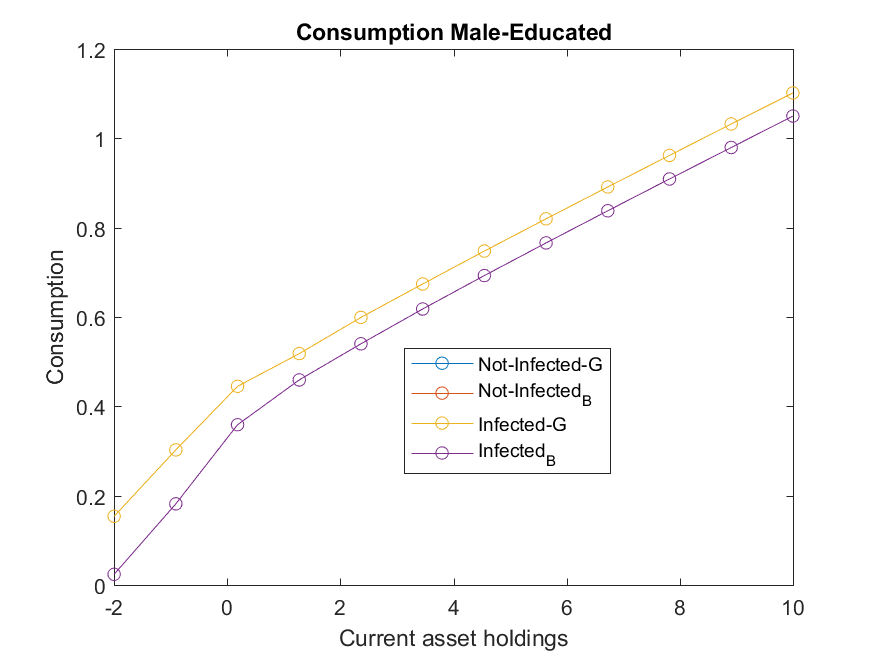
\includegraphics[angle=0,width=.5\textwidth]{figures/FIG2.png}   & 
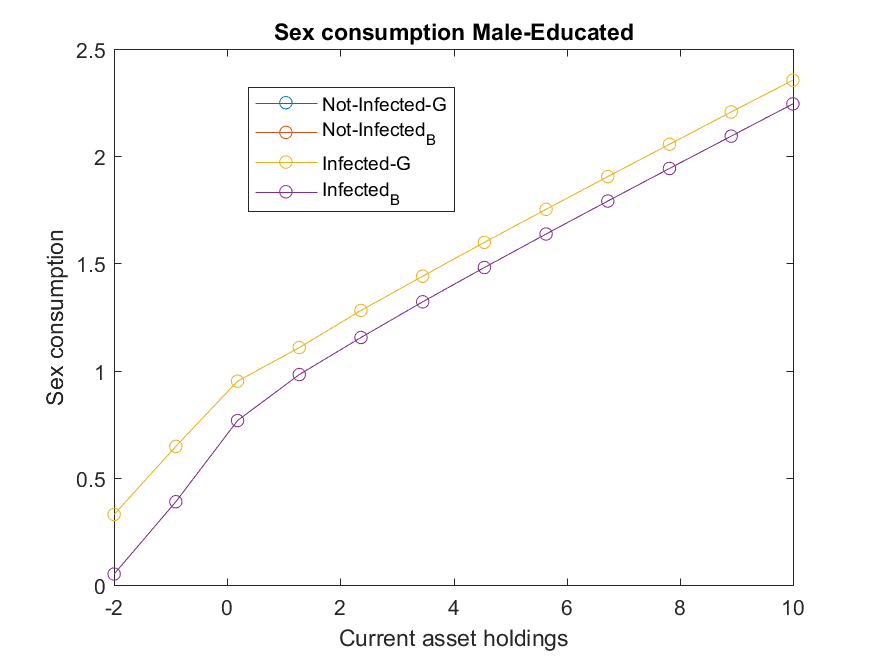
\includegraphics[angle=0,width=.5\textwidth]{figures/FIG4.png} \\
%\multicolumn{1}{c}{(a) Value function} &  
%\multicolumn{1}{c}{(b) Assets function} \\
\end{tabular}
\end{center}
\label{fig:2}
\end{figure}

\begin{figure}[H]
\caption{Policy Functions Educated Sellers}
\hspace{-2.0cm}
\begin{center}
\begin{tabular}{cc}
\multicolumn{1}{c}{(a) Value function} &  
\multicolumn{1}{c}{(b) Asset function} \\
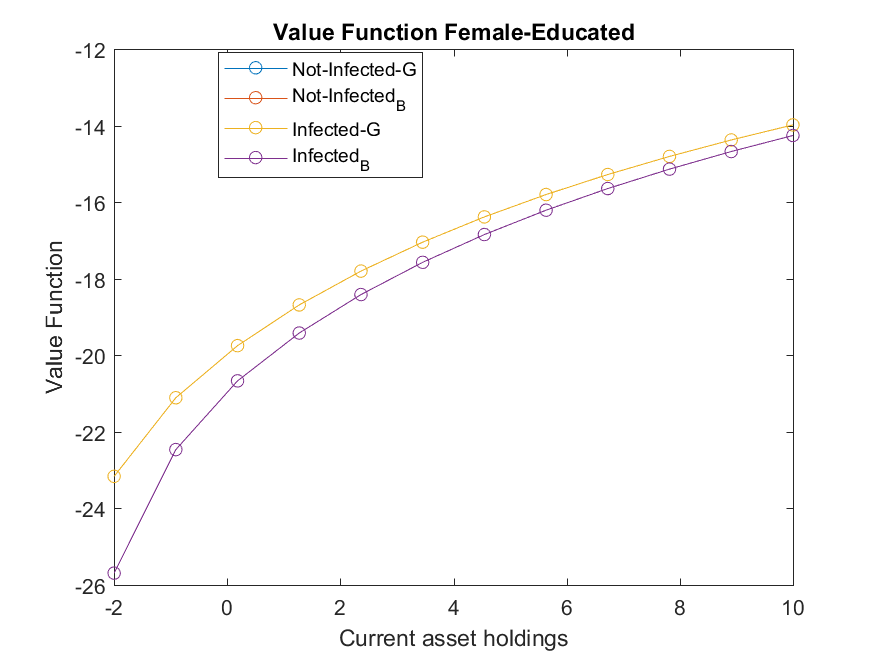
\includegraphics[angle=0,width=.5\textwidth]{figures/FIG5.png}   & 
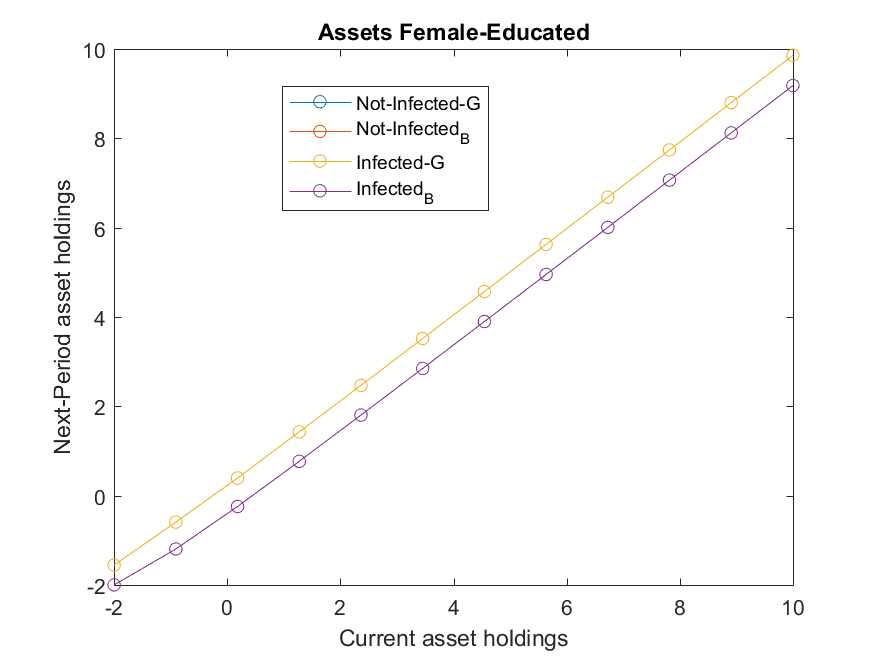
\includegraphics[angle=0,width=.5\textwidth]{figures/FIG7.png} \\
\multicolumn{1}{c}{(c) Consumption function} &  
\multicolumn{1}{c}{(d) Sex Production function } \\
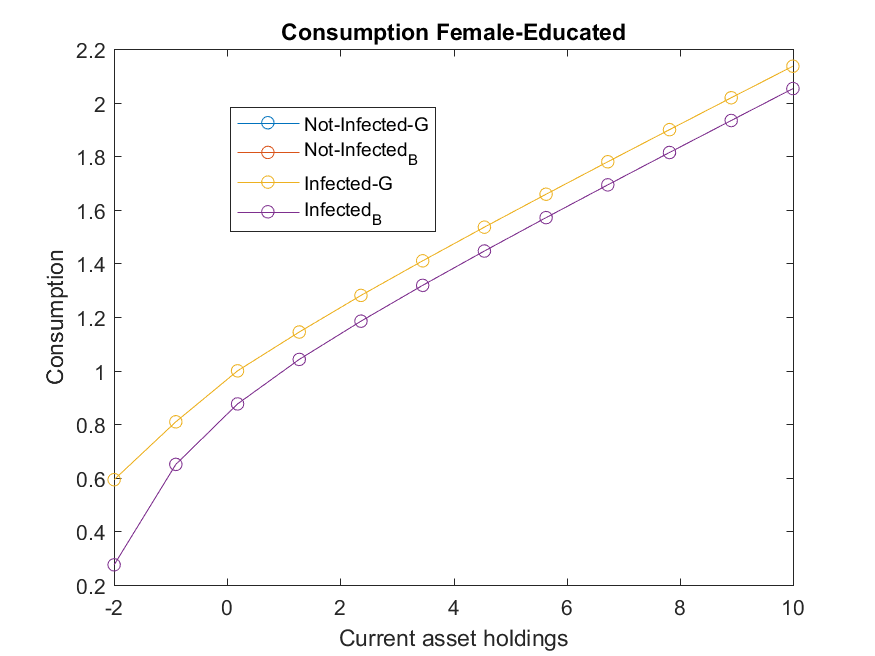
\includegraphics[angle=0,width=.5\textwidth]{figures/FIG6.png}   & 
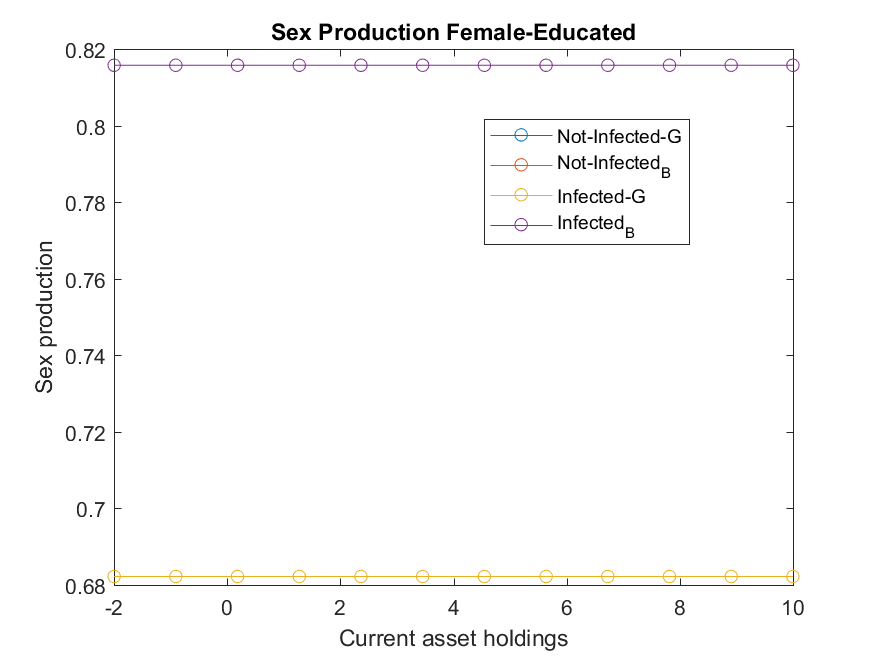
\includegraphics[angle=0,width=.5\textwidth]{figures/FIG8.png} \\
\end{tabular}
\end{center}
\label{fig:3}
\end{figure}



\begin{figure}[H]
\caption{Comparison plots}
\hspace{-2.0cm}
\begin{center}
\begin{tabular}{cc}
\multicolumn{1}{c}{(a) Asset Policy Functions} &  
\multicolumn{1}{c}{(b) Consumption Policy Functions} \\
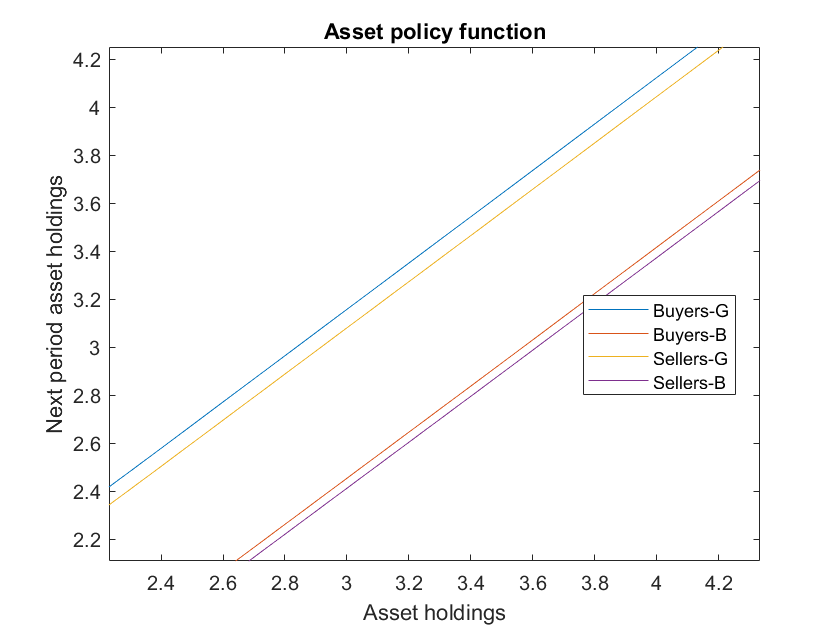
\includegraphics[angle=0,width=.5\textwidth]{figures/FIG11.png}   & 
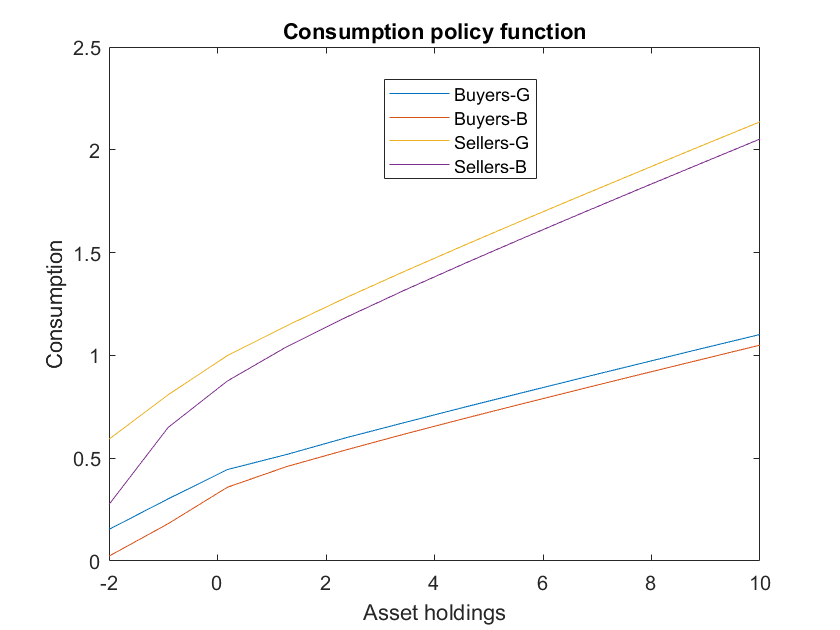
\includegraphics[angle=0,width=.5\textwidth]{figures/FIG12.png}\\ 
\multicolumn{2}{c}{(c) No Capital Income} \\  
%\multicolumn{2}{c}{(d) Equilibrium(repeated)} \\
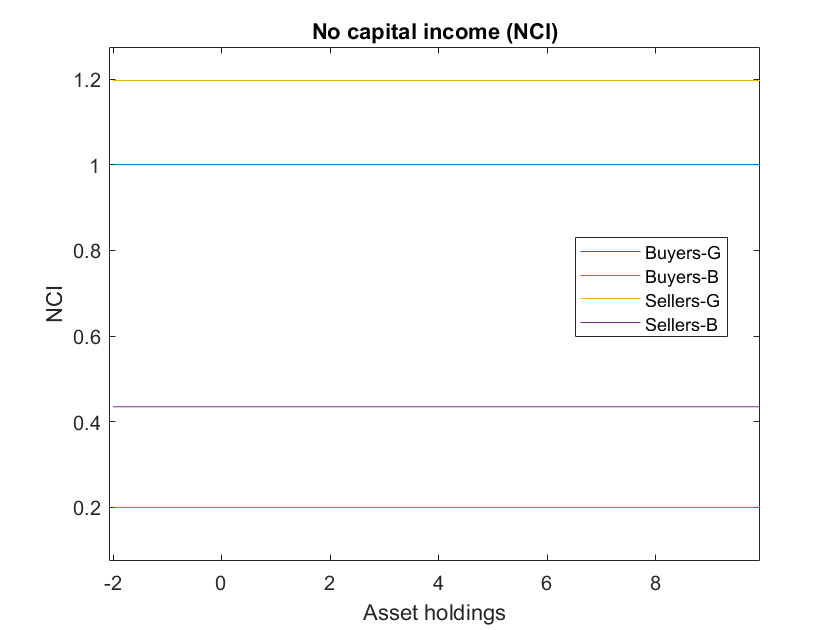
\includegraphics[angle=0,width=.5\textwidth]{figures/FIG13.png} 
%& 
%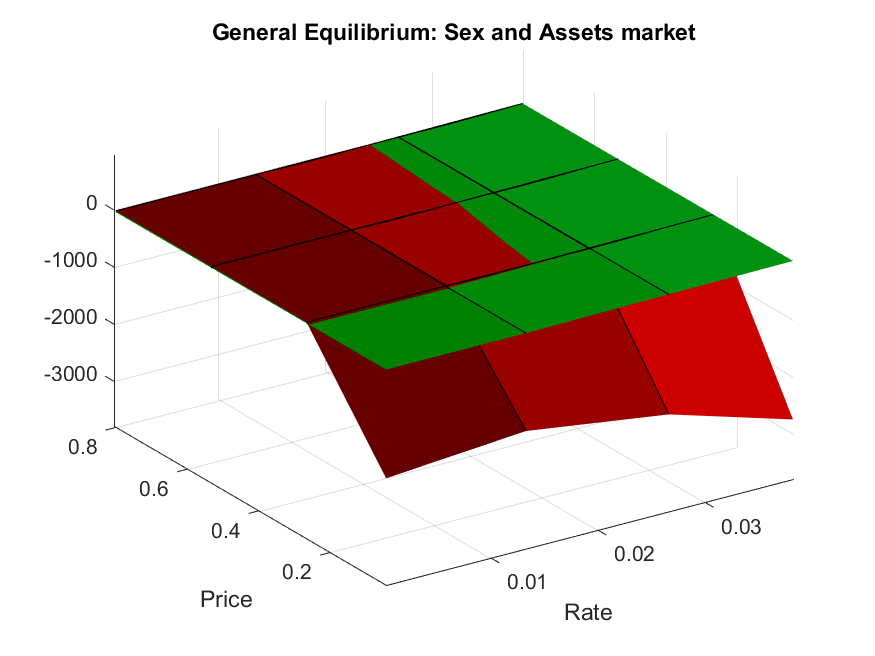
\includegraphics[angle=0,width=.5\textwidth]{figures/FIG_EQUILIBIUM3.png} 
\end{tabular}
\end{center}
\label{fig:5}
\end{figure}